\documentclass[12pt]{article}

\usepackage{amsmath}
\usepackage{amssymb}
\usepackage{calc}
\usepackage{units}
\usepackage{graphicx}
\usepackage[pdftex]{hyperref}
\usepackage{subfig}
\usepackage[margin=1in]{geometry}
\usepackage{listings}
\usepackage[numbers,sort&compress]{natbib}
\usepackage{bm}
\usepackage{paralist}
\usepackage[draft]{fixme}
\usepackage{textcomp}
\usepackage{yorkdefs}

\newcommand{\halflife}{\ensuremath{T_{\nicefrac{1}{2}}}\xspace}

\hypersetup{
  breaklinks=true,
  pdftitle={Alternating Current RL Circuits},
  pdfauthor={Kevin R. Lynch based on a lab by D.C.Jain}, 
  pdfsubject={Phyiscs, Electricity and magnetism},
  pdfkeywords={resistance, inductance, alternating current},
  pdflang={en-US},
}

\title{Alternating Current RL Circuits}
\author{}
%Kevin R. Lynch, based on an earlier lab by D.C.Jain
%\date{2012-03-16}
\date{}

\begin{document}

\maketitle

\section{Objectives}
\label{sec:objectives}

\begin{enumerate}
\item To understand the voltage/current phase behavior of RL circuits
  under applied alternating current voltages, and
\item To understand the current amplitude behavior of RL circuits
  under applied alternating current voltages.
\end{enumerate}

\section{Introduction}
\label{sec:introduction}

You have studied the behavior of RC circuits under both direct and
alternating current conditions.  The final passive component we must
consider is the \textit{inductor}.  The voltage across a capacitor is
proportional to the charge on it ($V(t) = q(t)/C$), and the voltage
across a resistor is proportional to the rate at which charge flows
through it ($V_R(t) = R \dd q(t)/\dd t$), while the voltage across the
inductor is proportional to the rate of change of the current
\begin{gather*}
  V_L(t) = - L \deriv{I(t)}{t}\ .
\end{gather*}
The minus sign indicates that the voltage across the inductor seeks to
minimize or negate the changing current.

\begin{figure}
  \centering
  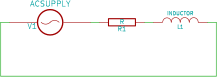
\includegraphics[width=2\textwidth/3]{figures/rl-circuit}
  \caption{The RL circuit.}
  \label{fig:rlcircuit}
\end{figure}
In a previous lab\footnote{\textit{Alternating Current RC Circuits}}
you studied the behavior of the RC circuit under alternating applied
(or AC) voltages.  Here, you will study the behavior of a similar
circuit where the capacitor is replaced with an \textit{inductor}; see
Figure~\ref{fig:rlcircuit}. 

The SI unit of inductance is the henry, with symbol \unit{H}:
\begin{gather*}
  \unit{H} = \unit{\Omega\, s} = \unit{\frac{kg\, m^2}{C^2}}\ .
\end{gather*}
The henry is named for Joseph Henry, an 18\textsuperscript{th} century
American contemporary of Michael Faraday.  Both men discovered
electromagnetic induction independently and contemporaneously.  Since
Faraday is honored in the unit of capacitance, Henry is honored with
the unit of inductance.

\section{Theory}
\label{sec:theory}

\begin{figure}
  \centering
  \includegraphics[width=2\textwidth/3]{figures/phase}
  \caption{A schematic of the phase difference between the applied
    voltage $V(t)$ and the derived current $I(t)$.}
  \label{fig:phase}
\end{figure}
Once again, let's analyze this circuit using Kirchoff's Rules.  As
always, you find
\begin{gather*}
  V_s(t) - V_R(t) - V_L(t) = 0\ ,
\end{gather*}
leading to the differential equation
\begin{gather*}
  \deriv{I(t)}{t} + \frac{R}{L} I(t) = \frac{V_s(t)}{L}\ .
\end{gather*}
This is, in all important ways, \textit{identical} to the behavior of
the charge on a capacitor.  The time constant for current changes is
here $\tau = L/R$.  Again, we solve the equation in all its
particulars in Appendix~\ref{sec:solutions}.  For a sinusoidally
varying source voltage
\begin{gather*}
  V_s(t) = V_s \cos\omega t\ ,
\end{gather*}
we find the current is again out of phase, but this time it
\textit{lags} the voltage (see Figure~\ref{fig:phase})
\begin{gather*}
  I(t) = \frac{V_s}{R} \frac{1}{\sqrt{1 + (\omega \tau)^2}}
  \cos(\omega t - \phi)\\
  V_R(t) = V_s \frac{1}{\sqrt{1 + (\omega \tau)^2}}
  \cos(\omega t - \phi)\\
  V_L(t) = V_s \frac{\omega \tau}{\sqrt{1 + (\omega \tau)^2}}
  \sin(\omega t - \phi)\ ,
\end{gather*}
where the phase is given by 
\begin{gather*}
  \tan \phi = \frac{\omega L}{R}\ .
\end{gather*}

Just as for the capacitor circuit, we can define and use the concept
of \textit{impedance} to predict the behavior of the circuit.  The
combination $\omega L$ has units of resistance, and we
define the \textit{inductive reactance} by
\begin{gather*}
  X_L = \omega L\ .
\end{gather*}
The phase is given by
\begin{gather*}
  \tan\phi = \frac{X_L}{R}\ ,
\end{gather*}
while the circuit impedance is given by
\begin{gather*}
  Z^2 = R^2 + X_L^2\ ,
\end{gather*}
which has all the same consequences for the voltage amplitudes as it
did for the $RC$ circuit.

\begin{figure}
  \centering
  \subfloat[][Phases]{
    \includegraphics[width=\textwidth/2-0.1in]{figures/frequency-phase}
  }
  \subfloat[][Voltage Amplitudes]{
    \includegraphics[width=\textwidth/2-0.1in]{figures/frequency-amplitudes}
  }
  \caption{The phase angle as a function of angular frequency is on
    the left, while the voltage amplitudes are displayed on the
    right.  In both cases, the frequency is normalized in units of
    $L/R$.  The phase is normalized to $\pi/2$, while the amplitudes
    are normalized to $V_s$.}
  \label{fig:frequency}
\end{figure}
Just as we did for the RC circuit, we can consider the behavior of
this circuit as a function of frequency.  In the limit that the
frequency goes to zero, the current will be steady state.  Since
steady state means ``no change'', the voltage across the inductor must
vanish, and the phase has to go to zero.  This is what we see in
Figure~\ref{fig:frequency}.  In the other extreme, with very high
frequencies, the current is changing very quickly, so the voltage will
all be visible across the inductor; again, this is what we see in
Figure~\ref{fig:frequency}.  Inductors become transparent at low
frequencies, and opaque at high frequencies, just the opposite of the
capacitor!  Compare the amplitude and phase response curves in
Figure~\ref{fig:frequency} with the same curves in the lab
\textit{Alternating Current RC Circuits}.

\section{Procedures}
\label{sec:procedures}

You should receive two multimeters (one of which should be a
BK-5460), an oscilloscope, a function generator, a
decade resistance box, and an inductor.

\begin{enumerate}
\item First, let's select component values for testing.  We don't have
  variable inductors available; instead, use the fixed inductor you
  have been provided, and record the inductance.  How much uncertainty
  do you think there is in this value?  Select a frequency between
  \unit[300]{Hz} and \unit[600]{Hz}.  Calculate $X_L$ and choose a
  value for $R \approx 1.2 X_L$.  Measure and record the value of $R$.
\item Configure the circuit for testing shown in
  Figure~\ref{fig:rlcircuit}.  Insert the Simpson multimeter to record
  the AC current; except in the last two steps of the procedure, make
  sure the current remains constant throughout the experiment.
\item Using the BK Precision meter, record the frequency $f$, and the
  RMS AC voltages across the signal generator $V_s$, the resistor
  $V_R$, and the inductor $V_L$.
\item \label{item:phase} Let's measure the phase shift between the
  current and applied voltage.  Connect the oscilloscope so as to
  measure the voltage across the resistor and signal generator; make
  sure the negtive inputs share a common reference point.  Make sure
  the two signal baselines are centered with respect to the horizontal
  and vertical axes of the oscilloscope, and adjust the voltage and
  time scales so that slightly more than one cycle of both waveforms
  is visible.  Measure the phase shift as you did in the previous lab.
  Increase the frequency by 50\%, and determine the phase shift again.
  Double the initial frequency, and repeat.
\item \label{item:current} Next, map out the amplitude of the current
  response.  Without changing $R$, vary the frequency over, say, ten
  points, and record the frequency, RMS voltage $V_s$ and RMS current
  $I$ at those points.  Record you observations of the amplitudes of
  $V_s$ and $V_R$ on the oscilloscope.
\end{enumerate}


\appendix

\section{Derivation of Solutions}
\label{sec:solutions}

The differential equation for the AC RL circuit is given in
Section~\ref{sec:theory}, and is nearly identical to the equations we
have studied in the DC RC and AC RC cases.  In fact, in the DC case,
we can just substitute $I(t)$ for $q(t)$ and $\tau = L/R$ for $\tau =
1/RC$, and we have the DC behavior of the RL circuit straightaway.  In
the discharging case
\begin{gather*}
  I(t) = I(t_0) e^{-(t-t_0)/\tau}\ ,
\end{gather*}
while in the charging case
\begin{gather*}
  I(t) = I(t_0) e^{-(t-t_0)/\tau} 
  + \frac{V_s}{R} \left(1-e^{-(t-t_0)/\tau} \right)\ .
\end{gather*}
Again, like the RC circuit, in the charging RL circuit, the initial
current ``stored'' in the inductor decays away, while the imposed
voltage ``stores'' a current in the inductor exponentially.

In the AC case, very little of the derivation changes between the RC
and RL circuits, provided we replace the time constants
appropriately.  If you follow through all the work from the RC lab,
you will find
\begin{multline*}
  I(t) = I(t_0) e^{-(t-t_0)/\tau} 
  - e^{-(t-t_0)/\tau} \frac{V_s}{R} \frac{1}{(1/\tau)^2 + \omega^2} 
  \left( \frac{1}{\tau} \cos \omega t_0 + \omega \sin \omega t_0 \right) \\
  + \frac{V_s}{R} \frac{1}{(1/\tau)^2 + \omega^2} 
  \left( \frac{1}{\tau} \cos \omega t + \omega \sin \omega t \right)\ .
\end{multline*}
Again, the first line is the transient response, while the second line
gives the steady state response.  Keeping only the steady state
response, the same techniques as last time give us the voltage
profiles and phases given in Section~\ref{sec:theory}.

\newpage

\section*{Pre-Lab Exercises}

Answer these questions as instructed on Blackboard; make sure to
submit them before your lab session!

\begin{enumerate}
\item Calculate the reactance of a $\unit[7]{H}$ capacitor at a
  frequency of \unit[250]{Hz}.
% 11 kOhm
\item If an RL circuit has a $\unit[50]{\Omega}$ resistor in series
  with a $\unit[7]{m H}$ inductor, what will its impedance be at
  \unit[500]{Hz}?
% 54.6 Ohm
\item An RL circuit has a $\unit[5]{k\Omega}$ resistor and a
  $\unit[1]{H}$ inductor.  At what frequency will the current
  lag the voltage by $\pi/4$?
% 800 Hz
\item An RL circuit has a $\unit[5]{k\Omega}$ resistor and a
  $\unit[1]{m H}$ inductor.  This circuit is driven by a
  \unit[100]{Hz} sine wave with \unit[1]{V} amplitude.  What is the
  amplitude of the current in the circuit?
% 0.20 mA
\end{enumerate}

\newpage

\section*{Post-Lab Exercises}

\begin{enumerate}
\item From your recorded inductance, and measured resistance and
  frequency, determine the reactance and impedance of your circuit.
  Make sure to estimate your uncertainties.  Determine the impedance
  experimentally via another method, taking care of the
  uncertaintites.% V_s/I
  Do you get the same results?
\item Estimate the uncertainties on the measured values of $V_s$,
  $V_L$, and $V_R$.  Are the three values consistent with each other?
  Explain what you mean by ``consistent''.
\item Describe qualitatively what happens to your signals when you
  vary the frequency.
\item From your measurements in Step~\ref{item:phase} of the
  procedure, determine the phase shift at each of the three measured
  frequencies, including an estimate of the uncertainty.  How do these
  compare to the theoretical predictions? 
\item Is your data from Step~\ref{item:current} consistent with the
  predictions of theory?  Specifically, do the voltage and current
  amplitudes measured by oscilloscope and by multimeter match, within
  uncertainties, and do they comport with theoretical expectations?
\item Discuss briefly whether you have met the objectives of the lab
  exercises.
\end{enumerate}

\end{document}

%%% Local Variables: 
%%% mode: latex
%%% TeX-master: t
%%% End: 
